\documentclass[11pt]{article}
\usepackage{october}
\usepackage{lineno}

\begin{document}

\title{Asymmetry and the Geometry of Reason}
% \author{Stefan Lukits}
\date{}
\maketitle

\section{Introduction}
\label{intr}

In the early 1970s, the dominant models for similarity in the
psychological literature were all geometric in nature. Distance
measures capturing similarity and dissimilarity between concepts
obeyed minimality, symmetry, and the triangle inequality. Then Amos
Tversky wrote a compelling paper undermining the idea that a metric
topology is the best model (see \scite{7}{tversky77}{}). Tversky gave
both theoretical and empirical reasons why similarity between concepts
did not fulfill minimality, symmetry, or the triangle inequality.
Geometry with its metric distance measures was not a helpful way to
model similarity. Tversky presented an alternative set-theoretic
approach which accommodated the data that could not be reconciled with
a geometry of similarity.

The aim of this paper is to help along a similar paradigm shift when
it comes to epistemic modeling of closeness or difference between
subjective probability distributions. The \qnull{geometry of reason}
(a term coined by Richard Pettigrew and Hannes Leitgeb, two of its
advocates) also violates reasonable expectation we may have toward an
acceptable model. Just as Tversky did, I will present a non-geometric
and asymmetric alternative: information theory. Information theory
fulfills the expectations that the geometry of reason violates and
incorporates basic Bayesian commitments to probabilism and standard
conditioning.

The geometry of reason refers to a view of epistemic utility in which
the underlying topology for credence functions (which may be
subjective probability distributions) on a finite number of events is
a metric space. 

\begin{quotex}
  \beispiel{Die Roll}\label{ex:dieroll} You are about to roll a
  six-sided die.
\end{quotex}

The set of non-negative credences that an agent assigns to the outcome
of the die roll in Example \ref{ex:dieroll} may be isomorphic to
$\mathbb{R}_{\geq{}0}^{6}$. If the agent fulfills the requirements of
probabilism, the isomorphism is to the more narrow set $\mathbb{S}^6$,
the six-dimensional simplex for which

\begin{equation}
  \label{eq:simplex}
  p_{1}+p_{2}+p_{3}+p_{4}+p_{5}+p_{6}=1.
\end{equation}

Since the isomorphism is to a metric space, there is a distance
relation between credence functions which can be used to formulate
axioms relating credences to epistemic utility and to justify or to
criticize contentious positions such as Bayesian conditionalization,
the principle of indifference, other forms of conditioning, or
probabilism itself (see especially works cited below by James Joyce;
Pettigrew and Leitgeb; David Wallace and Hilary Greaves). 

Before I introduce the notion of epistemic utility and some of the
substantial claims in the literature that epistemic utility together
with the geometry of reason give us, I want to spell out my claim that
(a) given an epistemic utility approach and some intuitive axioms, the
geometry of reason leads itself ad absurdum; and (b) there is a viable
alternative to the geometry of reason which avoids the problematic
implications: information theory. For information theory, as opposed
to the geometry of reason, the underlying topology for credence
functions is not a metric space. 

\begin{figure}[ht]
  \begin{flushright}
    \begin{minipage}[h]{.7\linewidth}
      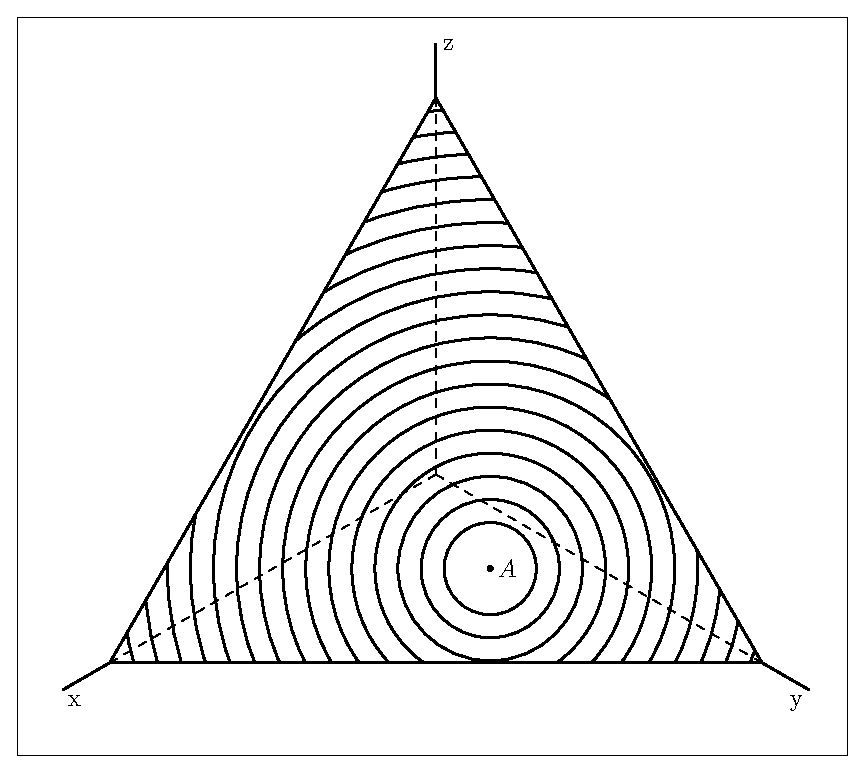
\includegraphics[width=\textwidth]{contourslp.eps}
      \caption{\footnotesize The simplex $\mathbb{S}^{3}$ in
        three-dimensional space $\mathbb{R}^{3}$ with contour lines
        corresponding to the geometry of reason around point $A$ in
        equation (\ref{eq:e6}). Points on the same contour line are
        equidistant from $A$ with respect to the Euclidean metric.
        Compare the contour lines here to figure
        (\ref{fig:contoursrj}). Note that this diagram and all the
        following diagrams are frontal views of the simplex.}
      \label{fig:contourslp}
    \end{minipage}
  \end{flushright}
\end{figure}

\begin{figure}[ht]
  \begin{flushright}
    \begin{minipage}[h]{.7\linewidth}
      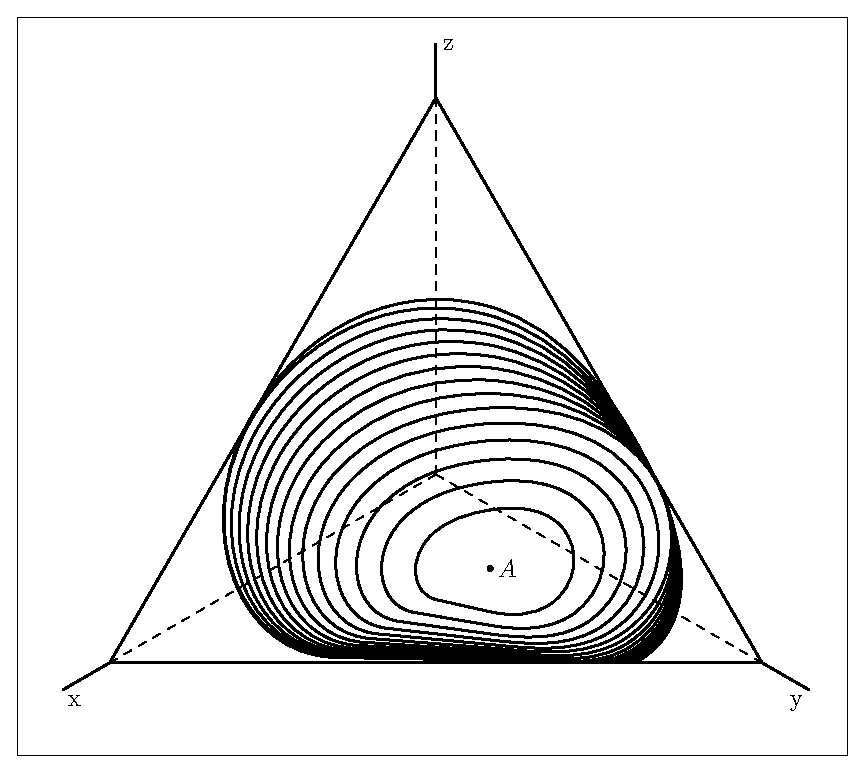
\includegraphics[width=\textwidth]{crj.eps}
      \caption{\footnotesize The simplex $\mathbb{S}^{3}$ with contour
        lines corresponding to information theory around point $A$ in
        equation (\ref{eq:e6}). Points on the same contour line are
        equidistant from $A$ with respect to the Kullback-Leibler
        divergence. The contrast to figure (\ref{fig:contourslp}) will
        become clear in much more detail in the body of the paper.
        Note that the contour lines of the geometry of reason are
        insensitive to the boundaries of the simplex, while the
        contour lines of information theory reflect them. The main
        argument of this paper is that information theory respects
        epistemic intuitions we have about asymmetry: proximity to
        extreme beliefs with very high or very low probability
        influences the topology that is at the basis of updating.}
      \label{fig:contoursrj}
    \end{minipage}
  \end{flushright}
\end{figure}

Before I argue for my claim, I want to give a brief overview of the
epistemic utility approach (contrasted most usefully with a pragmatic
utility approach) and look at the impressive results of applying the
geometry of reason. Epistemic utility in Bayesian epistemology has
attracted some attention in the past few years. Patrick Maher provides
a compelling acceptance-based account of epistemic utility (see
\scite{8}{maher93}{182--207}). Joyce, in \qeins{A Nonpragmatic
  Vindication of Probabilism,} defends probabilism supported by
partial-belief-based epistemic utility rather than the pragmatic
utility common in Dutch-book style arguments (see
\scite{7}{joyce98}{}). For Joyce, norms of gradational accuracy
characterize the epistemic utility approach to partial beliefs,
analogous to norms of truth for full beliefs.

Wallace and Greaves investigate epistemic utility functions along
\qnull{stability} lines and conclude that for everywhere stable
utility functions standard conditioning is optimal, while only
somewhere stable utility functions create problems for maximizing
expected epistemic utility norms (see \scite{7}{greaveswallace06}{};
and \scite{7}{pettigrew13}{}). Richard Pettigrew and Hannes Leitgeb
have published arguments that under certain assumptions probabilism
and standard conditioning (which together give epistemology a distinct
Bayesian flavour) minimize inaccuracy, thereby providing maximal
epistemic utility (see Leitgeb and Pettigrew,
\scite{11}{leitgebpettigrew10i}{} and
\scite{11}{leitgebpettigrew10ii}{}).

Leitgeb and Pettigrew show, given the geometry of reason and other
axioms inspired by Joyce (for example normality and dominance), that
in order to avoid epistemic dilemmas we must commit ourselves to a
Brier score measure of inaccuracy and subsequently to probabilism and
standard conditioning. Jeffrey conditioning (also called probability
kinematics) is widely considered to be a commonsense extension of
standard conditioning. On Leitgeb and Pettigrew's account, it fails to
provide maximal epistemic utility. Another type of conditioning, which
we will call LP conditioning, takes the place of Jeffrey conditioning.

The failure of Jeffrey conditioning to minimize inaccuracy on the
basis of the geometry of reason casts, by reductio, doubt on the
geometry of reason. I will show that LP conditioning, which the
geometry of reason entails, fails five commonsense expectations that
are reasonable to have for the kind of updating scenario that LP
conditioning addresses. To relate probability distributions to each
other geometrically, using the isomorphism between the set of
probability distributions on a finite event space $W$ with $|W|=n$ and
the $n$-dimensional simplex $\mathbb{S}^{n}\subset\mathbb{R}^{n}$, is
initially an arbitrary move. Leitgeb and Pettigrew do little to
substantiate a link between the geometry of reason and epistemic
utility on a conceptual level. It is the formal success of the model
that makes the geometry of reason attractive, but the failure of LP
conditioning to meet basic expectations undermines this success.

The question then remains whether we have a plausible candidate to
supplant the geometry of reason. The answer is yes: information theory
provides us with a measure of closeness between probability
distributions on a finite event space that has more conceptual appeal
than the geometry of reason, especially with respect to epistemic
utility---it is intuitively correct to relate coming-to-knowledge to
exchange of information. More persuasive than intuitions, however, is
the fact that information theory supports both standard conditioning
(see \scite{7}{williams80}{}) and the extension of standard
conditioning to Jeffrey conditioning (see
\scite{7}{catichagiffin06}{}; and \scite{7}{lukits15}{}), an extension
which is on the one hand commonsensical (see \scite{7}{wagner02}{})
and on the other hand formally continuous with the standard
conditioning which Leitgeb and Pettigrew have worked so hard to
vindicate nonpragmatically. LP conditioning is not continuous with
standard conditioning, one of the five expectations that LP
conditioning fails to meet.

There are four sections to come. Section \ref{eugr} describes the
geometry of reason and provides a brief overview of Leitgeb and
Pettigrew's strategy to give probabilism and standard conditioning a
foundation in epistemic utility. Section \ref{grit} gives a simple
example and a more general overview how the geometry of reason and
information theory give different results with respect to proximity
relations of probability distributions. The geometry of reason
supports LP conditioning, information theory supports Jeffrey
conditioning. Section \ref{fivex} demonstrates in detail how LP
conditioning violates five commonsense expectations and how Jeffrey
conditioning fulfills them. Section \ref{ascc} draws the conclusion
that information theory, not the geometry of reason, reflects in
formal terms what epistemic utility expresses in informal terms.

\section{Epistemic Utility and the Geometry of Reason}
\label{eugr}

There is more epistemic virtue for an agent in believing a truth
rather than not believing it and in not believing a falsehood rather
than believing it. Accuracy in full belief epistemology can be
measured by counting four sets, believed truths and falsehoods as well
as unbelieved truths and falsehoods, and somehow relating them to each
other such that epistemic virtue is rewarded and epistemic vice
penalized. Accuracy in partial belief epistemology must take a
different shape since as a \qnull{guess} all partial non-full beliefs
are off the mark so that they need to be appreciated as
\qnull{estimates} instead. Richard Jeffrey distinguishes between
guesses and estimates: a guess fails unless it is on target, whereas
an estimate succeeds depending on how close it is to the target.

The gradational accuracy needed for partial belief epistemology is
reminiscent of verisimilitude and its associated difficulties in the
philosophy of science (see \scite{7}{popper63}{};
\scite{7}{gemes07}{}; and \scite{7}{oddie13}{}). Both Joyce and
Leitgeb/Pettigrew propose axioms for a measure of gradational accuracy
for partial beliefs relying on the geometry of reason, i.e.\ the idea
of geometrical distance between distributions of partial belief
expressed in non-negative real numbers. In Joyce, the geometry of
reason is adopted without much reflection. Terms such as
\qnull{midpoint} between two distributions and
$\lambda{}b'+(1-\lambda)b''$ for distributions \qnull{between} two
distributions $b'$ and $b''$ are used freely. 

Leitgeb and Pettigrew muse about alternative geometries, especially
non-Euclidean ones. They suspect that these would be based on and in
the end reducible to Euclidean geometry but they do not entertain the
idea that they could drop the requirement of a metric topology
altogether (for the use of non-Euclidean geodesics in statistical
inference see \scite{7}{shunichi85}{}).Thomas Mormann explicitly warns
against the assumption that the metrics for a geometry of logic is
Euclidean by default, \qeins{All too often, we rely on geometric
  intuitions that are determined by Euclidean prejudices. The geometry
  of logic, however, does not fit the standard Euclidean metrical
  framework} (see \scite{8}{mormann05}{433}; also
\scite{7}{miller84}{}). Mormann concludes in his article
\qeins{Geometry of Logic and Truth Approximation,}

\begin{quotex}
  Logical structures come along with ready-made geometric structures
  that can be used for matters of truth approximation. Admittedly,
  these geometric structures differ from those we are accostumed [sic]
  with, namely, Euclidean ones. Hence, the geometry of logic is not
  Euclidean geometry. This result should not come as a big surprise.
  There is no reason to assume that the conceptual spaces we use for
  representing our theories and their relations have an Euclidean
  structure. On the contrary, this would appear to be an improbable
  coincidence. \scite{3}{mormann05}{453}
\end{quotex}

Leitgeb and Pettigrew define two notions, local and global inaccuracy,
and show that one must adopt a Brier score to measure inaccuracy in
order to avoid epistemic dilemmas trying to minimize inaccuracy on
both measures. To give the reader an idea what this looks like in
detail and for purposes of later exposition, I want to provide some of
the formal apparatus. Let $W$ be a set of worlds and $A\subseteq{}W$ a
proposition. Then

\begin{equation}
  \label{eq:linacc}
  I:P(W)\times{}W\times{}\mathbb{R}^{+}_{0}\rightarrow\mathbb{R}^{+}_{0}
\end{equation}

{\noindent}is a measure of local inaccuracy such that $I(A,w,x)$
measures the inaccuracy of the degree of credence $x$ with respect to
$A$ at world $w$. Let $\mbox{Bel}(W)$ be the set of all belief
functions (what we have been calling distributions of partial belief).
Then

\begin{equation}
  \label{eq:ginacc}
  G:W\times\mbox{Bel}(W)\rightarrow\mathbb{R}^{+}_{0}
\end{equation}

{\noindent}is a measure of global inaccuracy of a belief function $b$
at a possible world $w$ such that $G(w,b)$ measures the inaccuracy of
a belief function $b$ at world $w$.

Axioms such as normality and dominance guarantee that the only
legitimate measure of inaccuracy are Brier scores if one wants to
avoid epistemic dilemmas where one receives conflicting advice from
the local and the global measures. For local inaccuracy measures, this
means that there is $\lambda\in\mathbb{R}^{+}$ such that

\begin{equation}
  \label{eq:e1}
  I(A,w,x)=\lambda\left(\chi_{A}(w)-x\right)^{2}
\end{equation}

where $\chi_{A}$ is the characteristic function of $A$. For global
inaccuracy measures, this means that there is $\mu\in\mathbb{R}^{+}$
such that

\begin{equation}
  \label{eq:e2}
  G(w,b)=\mu\|w-b\|^{2}
\end{equation}

where $w$ and $b$ are represented by vectors and $\|u-v\|$ is the
Euclidean distance

\begin{equation}
  \label{eq:e3}
  \sqrt{\sum_{i=1}^{n}\left(u_{i}-v_{i}\right)^{2}}.
\end{equation}

We use (\ref{eq:e1}) to define expected local inaccuracy of degree of
belief $x$ in proposition $A$ by the lights of belief function $b$,
with respect to local inaccuracy measure $I$, and over the set $E$ of
epistemically possible worlds as follows:

\begin{equation}
  \label{eq:eli}
  \mbox{LExp}_{b}(I,A,E,x)=\sum_{w\in{}E}b(\{w\})I(A,w,x)=\sum_{w\in{}E}b(\{w\})\lambda\left(\chi_{A}(w)-x\right)^{2}.
\end{equation}

We use (\ref{eq:e2}) to define expected global inaccuracy of belief
function $b'$ by the lights of belief function $b$, with respect to
global inaccuracy measure $G$, and over the set $E$ of epistemically
possible worlds as follows:

\begin{equation}
  \label{eq:egi}
  \mbox{GExp}_{b}(G,E,b')=\sum_{w\in{}E}b(\{w\})G(w,b')=\sum_{w\in{}E}b(\{w\})\mu\|w-b\|^{2}.
\end{equation}

To give a flavour of how attached the axioms are to the geometry of
reason, here are Joyce's axioms called Weak Convexity and Symmetry,
which he uses to justify probabilism:

\begin{quotex}
  \textbf{Weak Convexity}: Let $m=(0.5b'+0.5b'')$ be the midpoint of the line
  segment between $b'$ and $b''$. If $I(b',\omega)=I(b'',\omega)$,
  then it will always be the case that $I(b',\omega)\geq{}I(m,\omega)$
  with identity only if $b'=b''$.
\end{quotex}

\begin{quotex}
  \textbf{Symmetry}: If $I(b',\omega)=I(b'',\omega)$, then for any
  $\lambda\in{}[0,1]$ one has\newline
  $I(\lambda{}b'+(1-\lambda)b'',\omega)=I((1-\lambda){}b'+\lambda{}b''),\omega)$.
\end{quotex}

Joyce advocates for these axioms in Euclidean terms, using
justifications such as \qeins{the change in belief involved in going
  from $b'$ to $b''$ has the same direction but a doubly greater
  magnitude than change involved in going from $b'$ to [the midpoint]
  $m$} (see \scite{8}{joyce98}{596}). In section \ref{Asymmetry}, I
will show that Weak Convexity holds, and Symmetry does not hold, in
\qnull{information geometry,} the topology generated by the
Kullback-Leibler divergence. The term information geometry is due to
Imre Csisz{\'a}r, who considers the Kullback-Leibler divergence an
asymmetric analogue of squared Euclidean distance and derives several
results that are intuitive information geometric counterparts of
standard results in Euclidean geometry (see chapter 3 of
\scite{7}{csiszarshields04}{}).

Leitgeb and Pettigrew's work is continuous with Joyce's work, but
significantly goes beyond it. Joyce wants much weaker assumptions and
would be leery of expected inaccuracies (\ref{eq:eli}) and
(\ref{eq:egi}), as they might presuppose the probabilism that Joyce
wants to justify. Leitgeb and Pettigrew investigate not only whether
probabilism and standard conditioning follow from gradational accuracy
based on the geometry of reason, but also uniform distribution (their
term for the claim of objective Bayesians that there is some principle
of indifference for ignorance priors) and Jeffrey conditioning. They
show that uniform distribution requires additional axioms which are
much less plausible than the ones on the basis of which they derive
probabilism and standard conditioning (see
\scite{8}{leitgebpettigrew10ii}{250f}); and that Jeffrey conditioning
does not fulfill Joyce's Norm of Gradational Accuracy (see
\scite{8}{joyce98}{579}), in short that it violates the pursuit of
epistemic virtue. Leitgeb and Pettigrew provide us with an alternative
method of updating for Jeffrey-type updating scenarios, which I will
call LP conditioning.

\begin{quotex}
  \beispiel{Sherlock Holmes}\label{ex:holmes} Sherlock Holmes
  attributes the following probabilities to the propositions $E_{i}$
  that $k_{i}$ is the culprit in a crime:
  $P(E_{1})=1/3,P(E_{2})=1/2,P(E_{3})=1/6$, where $k_{1}$ is Mr.\ R.,
  $k_{2}$ is Ms.\ S., and $k_{3}$ is Ms.\ T. Then Holmes finds some
  evidence which convinces him that $P'(F^{*})=1/2$, where $F^{*}$ is
  the proposition that the culprit is male and $P$ is relatively prior
  to $P'$. What should be Holmes' updated probability that Ms.\ S. is
  the culprit?
\end{quotex}

I will look at the recommendations of Jeffrey conditioning and LP
conditioning for Example \ref{ex:holmes} in the next section. For now,
we note that LP conditioning violates all of the following plausible
expectations for an amujus, an \qnull{alternative method of updating
  for Jeffrey-type updating scenarios.}

\begin{itemize}
\item \textsc{continuity} An amujus ought to be continuous with
  standard conditioning as a limiting case.
\item \textsc{regularity} An amujus ought not to assign a posterior
  probability of $0$ to an event which has a positive prior
  probability and about which the intervening evidence says nothing
  except that a strictly weaker event has a positive posterior
  probability.
\item \textsc{levinstein} An amujus ought not to give \qeins{extremely
    unattractive} results in a Levinstein scenario (see
  \scite{7}{levinstein12}{}).
\item \textsc{invariance} An amujus ought to be partition invariant.
\item \textsc{confirmation} An amujus ought to align with intuitions
  we have about degrees of confirmation.
\item \textsc{horizon} An amujus ought to exhibit the horizon effect
  which makes probability distributions which are nearer to extreme
  probability distributions appear to be closer to each other than
  they really are.
\item \textsc{asymmetry} An amujus ought to reflect epistemic
  asymmetries. Updating from one probability distribution to another
  may need to be reflected in a different proximity relation than vice
  versa.
\end{itemize}

We are faced with the choice of rejecting the geometry of reason or
accepting these unpleasant consequences. Fortunately, there is a live
alternative to the geometry of reason: information theory. Information
theory has its own axiomatic approach to justifying probabilism and
standard conditioning (see \scite{7}{shorejohnson80}{}). Furthermore,
information theory provides a justification for Jeffrey conditioning
and generalizes it (see \scite{7}{lukits15}{}). Information theory is
not a geometry of reason because it measures divergences, not
distances, between distributions of partial belief. The divergence of
$b''$ from $b'$ may not be equal to the divergence of $b'$ from $b''$.
Updating methods based on information theory (standard conditioning,
Jeffrey conditioning, the principle of maximum entropy) fulfill
expectations \textsc{continuity}, \textsc{invariance},
\textsc{levinstein}, \textsc{regularity}, and \textsc{asymmetry}.

Returning from general argument to mathematical detail, salient axioms
in Leitgeb and Pettigrew are both local and global Normality and
Dominance (see \scite{8}{leitgebpettigrew10i}{219}):

\begin{quotex}
  \textbf{Local Normality and Dominance}: If $I$ is a legitimate
  inaccuracy measure, then there is a strictly increasing function
  $f:\mathbb{R}^{+}_{0}\rightarrow\mathbb{R}^{+}_{0}$ such that, for
  any $A\in{}W$, $w\in{}W$, and $x\in\mathbb{R}^{+}_{0}$,
  \begin{equation}
    \label{eq:e4}
    I(A,w,x)=f\left(|\chi_{A}(w)-x|\right).
  \end{equation}
\end{quotex}

\begin{quotex}
  \textbf{Global Normality and Dominance}: If $G$ is a legitimate
  global inaccuracy measure, there is a strictly increasing function
  $g:\mathbb{R}^{+}_{0}\rightarrow\mathbb{R}^{+}_{0}$ such that, for
  all worlds $w$ and belief functions $b\in{}\mbox{Bel}(W)$,
  \begin{equation}
    \label{eq:e5}
  G(w,b)=g\left(\|w-b_{\mbox{{\tiny glo}}}\|\right).
  \end{equation}
\end{quotex}

Similarly to Joyce, these axioms are justified on the basis of
geometry, but this time more explicitly so:

\begin{quotex}
  Normality and Dominance [are] a consequence of taking seriously the
  talk of inaccuracy as \qnull{distance} from the truth, and [they
  endorse] the geometrical picture provided by Euclidean $n$-space as
  the correct clarification of this notion. As explained in section
  3.2, the assumption of this geometrical picture is one of the
  presuppositions of our account, and we do not have much to offer in
  its defense, except for stressing that we would be equally
  interested in studying the consequences of minimizing expected
  inaccuracy in a non-Euclidean framework. But without a doubt,
  starting with the Euclidean case is a natural thing to do.
\end{quotex}

The next section provides a simple example where the distance of
geometry and the divergence of information theory differ. With this
difference in mind, I will show how LP conditioning fails the six
expectations outlined above. The conclusion is that a rational agent
uses information theory, not the geometry of reason.

\section{Geometry of Reason versus Information Theory}
\label{grit}

Consider the following three points in three-dimensional space: 

\begin{equation}
  \label{eq:e6}
    A=\left(\frac{1}{3},\frac{1}{2},\frac{1}{6}\right) \hspace{.5in}
    B=\left(\frac{1}{2},\frac{3}{8},\frac{1}{8}\right)  \hspace{.5in}
    C=\left(\frac{1}{2},\frac{5}{12},\frac{1}{12}\right)
\end{equation}

All three are elements of the three-dimensional simplex
$\mathbb{S}^{3}$: their coordinates add up to $1$. Thus they represent
probability distributions over a partition of the event space into
three events. Now call $D_{\mbox{\tiny KL}}(A,B)$ the Kullback-Leibler
divergence of $B$ from $A$ defined as follows, where $a_{i}$ are the
Cartesian coordinates of $A$:

\begin{equation}
  \label{eq:e7}
  D_{\mbox{\tiny KL}}(A,B)=\sum_{i=1}^{3}a_{i}\ln\frac{a_{i}}{b_{i}}
\end{equation}

The Euclidean distance $\|A-B\|$ is defined as in equation
(\ref{eq:e3}). What is remarkable about the three points in
(\ref{eq:e6}) is that

\begin{equation}
  \label{eq:e8}
  \|A-C\|\approx{}0.204<\|A-B\|\approx{}0.212
\end{equation}

and

\begin{equation}
  \label{eq:e9}
  D_{\mbox{\tiny KL}}(A,B)\approx{}0.057<D_{\mbox{\tiny KL}}(A,C)\approx{}0.072.
\end{equation}

The Kullback-Leibler divergence and Euclidean distance give different
recommendations with respect to proximity. Assuming the global
inaccuracy measure presented in (\ref{eq:e2}) and $E=W$ (all possible
worlds are epistemically accessible),

\begin{equation}
  \label{eq:e8a}
  \mbox{GExp}_{A}(C)\approx{}0.653<\mbox{GExp}_{A}(B)\approx{}0.656.
\end{equation}

\begin{figure}[ht]
  \begin{flushright}
    \begin{minipage}[h]{.7\linewidth}
      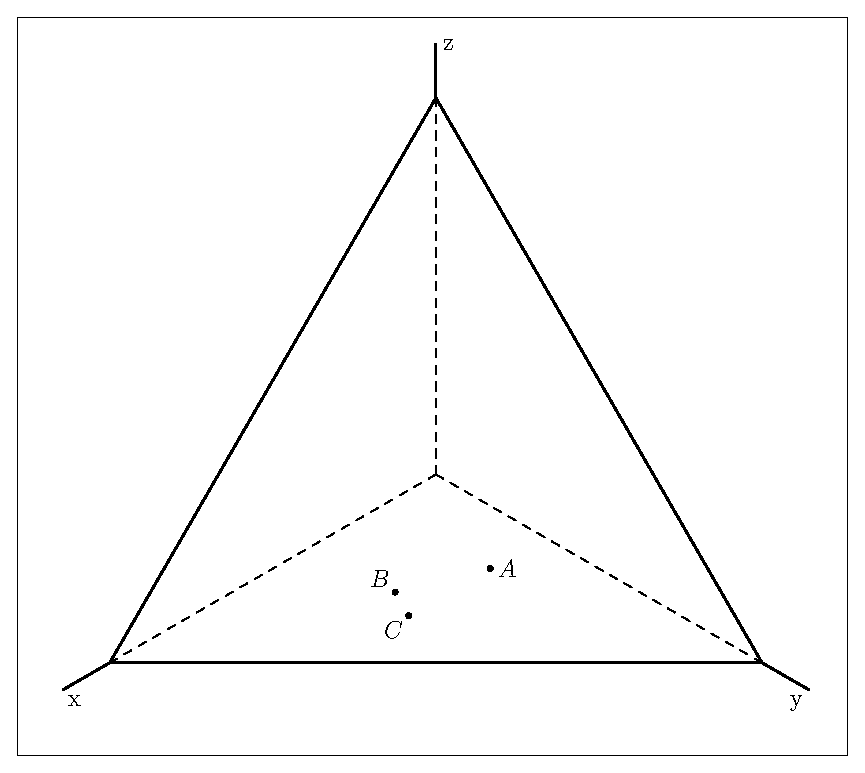
\includegraphics[width=\textwidth]{threepoints.eps}
      \caption{\footnotesize The simplex $\mathbb{S}^{3}$ in
        three-dimensional space $\mathbb{R}^{3}$ with points $A,B,C$
        as in equation (\ref{eq:e6}). Note that geometrically speaking
        $C$ is closer to $A$ than $B$ is. Using the Kullback-Leibler
        divergence, however, $B$ is closer to $A$ than $C$ is. The
        reason is asymmetry in information theory, which accords with
        our intuitions about epistemic space.}
      \label{fig:threepoints}
    \end{minipage}
  \end{flushright}
\end{figure}

Global inaccuracy reflects the Euclidean proximity relation, not the
recommendation of information theory. If $A$ corresponds to my prior
and my evidence is such that I must change the first coordinate to
$1/2$ and nothing stronger, then information theory via the
Kullback-Leibler divergence recommends the posterior corresponding to
$B$; and the geometry of reason as expounded in Leitgeb and Pettigrew
recommends the posterior corresponding to $C$.

There are several things going on here that need some explanation.
First, we note that for Leitgeb and Pettigrew, expected global
inaccuracy of $b'$ is always evaluated by the lights of another
partial belief distribution $b$. This may sound counterintuitive.
Should we not evaluate $b'$ by its own lights? It is part of a larger
Bayesian commitment that partial belief distributions are not created
ex nihilo. They can also not be evaluated for inaccuracy ex nihilo.
Leitgeb and Pettigrew say very little about this, but it appears that
there is a deeper problem here with the flow of diachronic updating.
The classic Bayesian picture is one of moving from a relatively prior
probability distribution to a posterior distribution (distinguish
relatively prior probability distributions, which precede posterior
probability distributions in updating, from absolutely prior
probability distributions, which are ignorance priors in the sense
that they are not the resulting posteriors of previous updating). This
is nicely captured by standard conditioning, Bayes' formula, and
updating on the basis of information theory (the Kullback-Leibler
divergence reflects this flow by asymmetries which we will bring up
again below).

The geometry of reason and notions of accuracy based on it sit
uncomfortably with this idea of flow, as the suggestion is that
partial belief distributions are evaluated on their accuracy without
reference to a prior probability distributions---why should the
accuracy or epistemic virtue of a posterior probability distribution
depend on a prior probability distribution which has already been
debunked by the evidence? I agree with Leitgeb and Pettigrew that
there is no alternative here but to evaluate the posterior by the
lights of the prior. Not doing so would saddle us with Carnap's
Straight Rule, where priors are dismissed as irrelevant (see
\scite{8}{carnap52}{40ff}). Yet we shall note that a justification of
evaluating a belief function's accuracy by the lights of another
belief function is a lot less persuasive than the way Bayesians and
information theory integrate prior distributions into forming
posterior distributions by virtue of an asymmetric flow of
information.

Second, I want to outline how Leitgeb and Pettigrew arrive at
posterior probability distributions in Jeffrey-type updating
scenarios. I will call their method LP conditioning. 

\begin{quotex}
  \beispiel{Abstract Holmes}\label{ex:abstract} Consider a possibility
  space $W=E_{1}\cup{}E_{2}\cup{}E_{3}$ (the $E_{i}$ are sets of
  states which are pairwise disjoint and whose union is $W$) and a
  partition $\mathcal{F}$ of $W$ such that
  $\mathcal{F}=\{F^{*},F^{**}\}=\{E_{1},E_{2}\cup{}E_{3}\}$.
\end{quotex}

Let $P$ be the prior probability function on $W$ and $P'$ the
posterior. I will keep the notation informal to make this simple, not
mathematically precise. Jeffrey-type updating scenarios give us new
information on the posterior probabilities of partitions such as
$\mathcal{F}$. In Example \ref{ex:abstract}, let

\begin{equation}
  \label{eq:priors}
  \begin{array}{rcl}
    P(E_{1})&=&1/3 \\
    P(E_{2})&=&1/2 \\
    P(E_{3})&=&1/6
  \end{array}
\end{equation}

and the new evidence constrain $P'$ such that
$P'(F^{*})=1/2=P'(F^{**})$.

Jeffrey conditioning works on the following intuition, which elsewhere
I have called Jeffrey's updating principle \textsc{jup} (see also
\scite{7}{wagner02}{}) and where the posterior probabilities
conditional on the partition elements equal the prior probabilities
conditional on the partition elements (since we have no information in
the evidence that they should have changed):

\begin{align}
  \label{eq:jc}
  &P'_{\mbox{\tiny JC}}(E_{i})&=&P'(E_{i}|F^{*})P'(F^{*})+P'(E_{i}|F^{**})P'(F^{**})\notag \\
  &&=&P(E_{i}|F^{*})P'(F^{*})+P(E_{i}|F^{**})P'(F^{**})
\end{align}

Jeffrey conditioning is controversial (for an introduction to Jeffrey
conditioning see \scite{7}{jeffrey65}{}; for its statistical and
formal properties see \scite{7}{diaconiszabell82}{}; for a pragmatic
vindication of Jeffrey conditioning see \scite{7}{armendt80}{}, and
\scite{7}{skyrms86}{}; for criticism see
\scite{7}{howsonfranklin94}{}). Information theory, however, supports
Jeffrey conditioning. Leitgeb and Pettigrew show that Jeffrey
conditioning does not in general pick out the minimally inaccurate
posterior probability distribution. If the geometry of reason as
presented in Leitgeb and Pettigrew is sound, this would constitute a
powerful criticism of Jeffrey conditioning. Leitgeb and Pettigrew
introduce an alternative to Jeffrey conditioning, which we have called
LP conditioning. It proceeds as follows for Example \ref{ex:abstract}
and in general provides the minimally inaccurate posterior probability
distribution in Jeffrey-type updating scenarios.

Solve the following two equations for $x$ and $y$:

\begin{equation}
  \label{eq:lpce}
  \begin{array}{rcl}
    P(E_{1})+x&=&P'(F^{*}) \\
    P(E_{2})+y+P(E_{3})+y&=&P'(F^{**})
  \end{array}
\end{equation}

and then set

\begin{equation}
  \label{eq:lpcf}
  \begin{array}{rcl}
    P'_{\mbox{\tiny LP}}(E_{1})&=&P(E_{1})+x \\
    P'_{\mbox{\tiny LP}}(E_{2})&=&P(E_{2})+y \\
    P'_{\mbox{\tiny LP}}(E_{3})&=&P(E_{3})+y
  \end{array}
\end{equation}

For the more formal and more general account see
\scite{8}{leitgebpettigrew10ii}{254}. The results for Example
\ref{ex:abstract} are:

\begin{equation}
  \label{eq:lpcres}
  \begin{array}{rcl}
    P'_{\mbox{\tiny LP}}(E_{1})&=&1/2 \\
    P'_{\mbox{\tiny LP}}(E_{2})&=&5/12 \\
    P'_{\mbox{\tiny LP}}(E_{3})&=&1/12
  \end{array}
\end{equation}

Compare these results to the results of Jeffrey conditioning:

\begin{equation}
  \label{eq:jcres}
  \begin{array}{rcl}
    P'_{\mbox{\tiny JC}}(E_{1})&=&1/2 \\
    P'_{\mbox{\tiny JC}}(E_{2})&=&3/8 \\
    P'_{\mbox{\tiny JC}}(E_{3})&=&1/8
  \end{array}
\end{equation}

Note that (\ref{eq:priors}), (\ref{eq:jcres}), and (\ref{eq:lpcres})
correspond to $A,B,C$ in (\ref{eq:e6}). 

\section{Six Expectations}
\label{fivex}

It remains to provide more detail for the six expectations and to
show how LP conditioning violates them. 

\subsection{Continuity}
\label{Continuity}

LP conditioning violates \textsc{continuity} because standard
conditioning gives a different recommendation than a parallel sequence
of Jeffrey-type updating scenarios which get arbitrarily close to
standard event observation. This is especially troubling considering
how important the case for standard conditioning is to Leitgeb and
Pettigrew.

To illustrate a \textsc{continuity} violation, consider the case where
Sherlock Holmes reduces his credence that the culprit was male to
$\varepsilon_{n}=1/n$ for $n=4,5,\ldots$. The sequence
$\varepsilon_{n}$ is not meant to reflect a case where Sherlock Holmes
becomes successively more certain that the culprit was female. It is
meant to reflect countably many parallel scenarios which only differ
by the degree to which Sherlock Holmes is sure that the culprit was
female. These parallel scenarios give rise to a parallel sequence (as
opposed to a successive sequence) of updated probabilities
$P'_{\mbox{\tiny LP}}(F^{**})$ and another sequence of updated
probabilities $P'_{\mbox{\tiny JC}}(F^{**})$ ($F^{**}$ is the
proposition that the culprit is female). As $n\rightarrow\infty$, both
of these sequences go to one.

Straightforward conditionalization on the evidence that \qnull{the
  culprit is female} gives us 

\begin{equation}
  \label{eq:sherlockcontsc}
  \begin{array}{rcl}
  P'_{\mbox{\tiny SC}}(E_{1})&=&0\\
  P'_{\mbox{\tiny SC}}(E_{2})&=&3/4\\
  P'_{\mbox{\tiny SC}}(E_{3})&=&1/4.
\end{array}
\end{equation}

Letting $n\rightarrow\infty$ for Jeffrey conditioning yields

\begin{equation}
  \label{eq:sherlockcontjc}
  \begin{array}{rcccl}
  P'_{\mbox{\tiny JC}}(E_{1})&=&1/n&\rightarrow&0\\
  P'_{\mbox{\tiny JC}}(E_{2})&=&3(n-1)/4n&\rightarrow&3/4\\
  P'_{\mbox{\tiny JC}}(E_{3})&=&(n-1)/4n&\rightarrow&1/4,
\end{array}
\end{equation}

whereas letting $n\rightarrow\infty$ for LP conditioning yields

\begin{equation}
  \label{eq:sherlockcontlp}
  \begin{array}{rcccl}
  P'_{\mbox{\tiny LP}}(E_{1})&=&1/n&\rightarrow&0\\
  P'_{\mbox{\tiny LP}}(E_{2})&=&(4n-1)/6n&\rightarrow&2/3\\
  P'_{\mbox{\tiny LP}}(E_{3})&=&(2n-1)/6n&\rightarrow&1/3.
\end{array}
\end{equation}

LP conditioning violates \textsc{continuity}.

\subsection{Regularity}
\label{Regularity}

LP conditioning violates \textsc{regularity} because formerly positive
probabilities can be reduced to $0$ even though the new information in
the Jeffrey-type updating scenario makes no such requirements (as is
usually the case for standard conditioning). Ironically, Jeffrey-type
updating scenarios are meant to be a better reflection of real-life
updating because they avoid extreme probabilities. 

The violation becomes especially egregious if we are already somewhat
sympathetic to an information-based account: the amount of information
required to turn a non-extreme probability into one that is extreme
($0$ or $1$) is infinite. Whereas the geometry of reason considers
extreme probabilities to be easily accessible by non-extreme
probabilities under new information (much like a marble rolling off a
table or a bowling ball heading for the gutter), information theory
envisions extreme probabilities more like an event horizon. The nearer
you are to the extreme probabilities, the more information you need to
move on. For an observer, the horizon is never reached.

\begin{quotex}
  \beispiel{Regularity Holmes}\label{ex:regularity} Everything is as
  in Example \ref{ex:holmes}, except that Sherlock Holmes becomes
  confident to a degree of $2/3$ that Mr.\ R is the culprit and
  updates his relatively prior probability distribution in
  (\ref{eq:priors}).
\end{quotex}

Then his posterior probabilities look as follows:

\begin{equation}
  \label{eq:sherlockposteriorjcreg}
  \begin{array}{rcl}
  P'_{\mbox{\tiny JC}}(E_{1})&=&2/3\\
  P'_{\mbox{\tiny JC}}(E_{2})&=&1/4\\
  P'_{\mbox{\tiny JC}}(E_{3})&=&1/12
\end{array}
\end{equation}

\begin{equation}
  \label{eq:sherlockposteriorlpreg}
  \begin{array}{rcl}
  P'_{\mbox{\tiny LP}}(E_{1})&=&2/3\\
  P'_{\mbox{\tiny LP}}(E_{2})&=&1/3\\
  P'_{\mbox{\tiny LP}}(E_{3})&=&0
\end{array}
\end{equation}

With LP conditioning, Sherlock Holmes' subjective probability that
Ms.\ T is the culprit in Example \ref{ex:regularity} has been reduced
to zero. No finite amount of information could bring Ms.\ T back into
consideration as a culprit in this crime, and Sherlock Holmes should
be willing to bet any amount of money against a penny that she is not
the culprit---even though his evidence is nothing more than an
increase in the probability that Mr.\ R is the culprit.

LP conditioning violates \textsc{regularity}.

\subsection{Levinstein}
\label{Levinstein}

LP conditioning violates \textsc{levinstein} because of \qeins{the
  potentially dramatic effect [LP conditioning] can have on the
  likelihood ratios between different propositions}
\scite{3}{levinstein12}{419}. Consider Benjamin Levinstein's example:

\begin{quotex}
  \beispiel{Levinstein's Ghost}\label{ex:levinstein} There is a car
  behind an opaque door, which you are almost sure is blue but which
  you know might be red. You are almost certain of materialism, but
  you admit that there's some minute possibility that ghosts exist.
  Now the opaque door is opened, and the lighting is fairly good. You
  are quite surprised at your sensory input: your new credence that
  the car is red is very high.
\end{quotex}

Jeffrey conditioning leads to no change in opinion about ghosts. Under
LP conditioning, however, seeing the car raises the probability that
there are ghosts to an astonishing 47\%, given Levinstein's reasonable
priors. Levinstein proposes a logarithmic inaccuracy measure as a
remedy to avoid violation of \textsc{levinstein} (vaguely related to
the Kullback-Leibler divergence), but his account falls far short of
the formal scope, substance, and integrity of information theory.
As a special case of applying a Levinstein-type logarithmic inaccuracy
measure, information theory does not violate \textsc{levinstein}.

\subsection{Invariance}
\label{Invariance}

LP conditioning violates \textsc{invariance} because two agents who
have identical credences with respect to a partition of the event
space may disagree about this partition after LP conditioning, even
when the Jeffrey-type updating scenario provides no new information
about the more finely grained partitions on which the two agents
disagree. 

\begin{quotex}
  \beispiel{Jane Marple}\label{ex:marple} Jane Marple is on the same
  case as Sherlock Holmes in Example \ref{ex:holmes} and arrives at
  the same relatively prior probability distribution as Sherlock
  Holmes (we will call Jane Marple's relatively prior probability
  distribution $Q$ and her posterior probability distribution $Q'$).
  Jane Marple, however, has a more fine-grained probability assignment
  than Sherlock Holmes and distinguishes between the case where Ms.\ S
  went to boarding school with her, of which she has a vague memory,
  and the case where Ms.\ S did not and the vague memory is only about
  a fleeting resemblance of Ms.\ S with another boarding school mate.
  Whether or not Ms.\ S went to boarding school with Jane Marple is
  completely beside the point with respect to the crime, and Jane
  Marple considers the possibilities equiprobable whether or not Ms.\
  S went to boarding school with her.
\end{quotex}

Let $E_{2}\equiv{}E_{2}^{*}\vee{}E_{2}^{**}$, where $E_{2}^{*}$ is the
proposition that Ms.\ S is the culprit and she went to boarding school
with Jane Marple and $E_{2}^{**}$ is the proposition that Ms.\ S is
the culprit and she did not go to boarding school with Jane Marple.
Then

\begin{equation}
  \label{eq:marpleprior}
  \begin{array}{rcl}
  Q(E_{1})&=&1/3\\
  Q(E_{2}^{*})&=&1/4\\
  Q(E_{2}^{**})&=&1/4\\
  Q(E_{3})&=&1/6.
\end{array}
\end{equation}

Now note that while Sherlock Holmes and Jane Marple agree on the
relevant facts of the criminal case (who is the culprit?) in their
posterior probabilities if they use Jeffrey conditioning,

\begin{equation}
  \label{eq:sherlockposteriorjc}
  \begin{array}{rcl}
  P'_{\mbox{\tiny JC}}(E_{1})&=&1/2\\
  P'_{\mbox{\tiny JC}}(E_{2})&=&3/8\\
  P'_{\mbox{\tiny JC}}(E_{3})&=&1/8
\end{array}
\end{equation}

\begin{equation}
  \label{eq:marpleposteriorjc}
  \begin{array}{rcl}
  Q'_{\mbox{\tiny JC}}(E_{1})&=&1/2\\
  Q'_{\mbox{\tiny JC}}(E_{2}^{*})&=&3/16\\
  Q'_{\mbox{\tiny JC}}(E_{2}^{**})&=&3/16\\
  Q'_{\mbox{\tiny JC}}(E_{3})&=&1/8
\end{array}
\end{equation}

they do not agree if they use LP conditioning,

\begin{equation}
  \label{eq:sherlockposteriorlp}
  \begin{array}{rcl}
  P'_{\mbox{\tiny LP}}(E_{1})&=&1/2\\
  P'_{\mbox{\tiny LP}}(E_{2})&=&5/12\\
  P'_{\mbox{\tiny LP}}(E_{3})&=&1/12
\end{array}
\end{equation}

\begin{equation}
  \label{eq:marpleposteriorlp}
  \begin{array}{rcl}
  Q'_{\mbox{\tiny LP}}(E_{1})&=&1/2\\
  Q'_{\mbox{\tiny LP}}(E_{2}^{*})&=&7/36\\
  Q'_{\mbox{\tiny LP}}(E_{2}^{**})&=&7/36\\
  Q'_{\mbox{\tiny LP}}(E_{3})&=&1/9.
\end{array}
\end{equation}

LP conditioning violates \textsc{invariance}.

Postscript: One particular problem with the lack of invariance for LP
conditioning is how zero-probability events should be included in the
list of prior probabilities that determines the value of the posterior
probabilities. Consider

\begin{equation}
  \label{eq:reginvone}
  \begin{array}{rcl}
  P(X_{1})&=&0\\
  P(X_{2})&=&0.3\\
  P(X_{3})&=&0.6\\
  P(X_{4})&=&0.1\\
\end{array}
\end{equation}

That $P(X_{1})=0$ may be a consequence of standard conditioning in a
previous step. Now the agent learns that $P'(X_{3}\vee{}X_{4})=0.5$.
Should the agent update on the list presented in (\ref{eq:reginvone})
or on the following list:

\begin{equation}
  \label{eq:reginvtwo}
  \begin{array}{rcl}
  P(X_{2})&=&0.3\\
  P(X_{3})&=&0.6\\
  P(X_{4})&=&0.1\\
\end{array}
\end{equation}

Whether you update on (\ref{eq:reginvone}) or (\ref{eq:reginvtwo})
makes no difference to Jeffrey conditioning, but due to the lack of
invariance it makes a difference to LP conditioning, so the geometry
of reason needs to find a principled way to specify the appropriate
prior probabilities. The only non-arbitrary way to do this is either
to include or to exclude all zero probability events on the list. This
strategy, however, sounds ill-advised unless one signs on to a
stronger version of \textsc{regularity} and requires that only a fixed
set of events can have zero probabilities (such as logical
contradictions)---but then LP conditioning runs afoul of
\textsc{regularity} and takes us out of the frying pan into the fire.

\subsection{Confirmation}
\label{Confirmation}

See degree of confirmation in jeco.org.

\subsection{Horizon}
\label{Horizon}

\begin{quotex}
  \beispiel{Undergraduate Complaint}\label{ex:complaint} An
  undergraduate student complains to the department head that the
  professor will not reconsider an 89\% grade (which misses an A+ by
  one percent) when reconsideration was given to other students with a
  67\% grade (which misses a B- by one percent).
\end{quotex}

Intuitions may diverge, but the professor's reasoning is as follows.
To improve a 60\% paper by ten percent is easily accomplished: having
your roommate check your grammar, your spelling, and your line of
argument will sometimes do the trick. It is incomparably more
difficult to improve an 85\% paper by ten percent: it may take doing a
PhD to turn a student who writes the former into a student who writes
the latter. Consequently, the step from 89\% to 90\% is much greater
than the step from 67\% to 68\%.

Similarly, probability distributions with near-extreme (though still
regular) probabilities are informationally further apart from each
other than more mainstream probability distributions, even when the
Euclidean distances are the same. Consider the following five rules,
all of which are merely illustrations of the horizon effect.

\begin{description}
\item[Kitchen Rule] It is easier to get things out of the kitchen
  cabinet than it is to put them back in. In terms of information, it
  is more costly to move (by probability kinematics, for example) from
  a probability distribution with higher entropy (closer to the centre
  of the simplex) to a probability distribution with lower entropy
  (closer to the periphery of the simplex) than the reverse. The
  difference is subtle, not pronounced. It takes just a little more to
  almost exclude a heretofore plausible hypothesis (maybe from 1/2 to
  1/100) than it does to include a heretofore implausible hypothesis
  (maybe from 1/100 to 1/2).
\item[Similarity Rule] Defaults introduce asymmetries. Tversky
  extensively illustrates this rule (see \scite{7}{tversky77}{}). An
  ellipse, for example, is more similar to a circle than a circle is
  similar to an ellipse, at least psychologically. As in the Kitchen
  Rule, the difference can be subtle. However, it speaks in favour of
  information theory that it reflects this difference in numerically
  subtle ways, compared to the geometry of reason which ignores it.
  Similarity of concepts is like similarity of subjective probability
  distributions in the sense that they both exhibit features of
  asymmetry which are in tension with the initial appeal of using
  metric distance measures to model them. 
\item[Field Rule] For the geometry of reason, the borders of the
  simplex introduce a simple boundary condition (not dissimilar to
  boundary conditions for Lagrange Multiplier problems, see
  \scite{7}{bertsekas82}{}). For information theory, the presence of
  extreme probabilities at the border of the simplex introduces a
  topology that is highly sensitive to where these borders are. The
  asymmetry claim is that a simplex of subjective probability
  distributions is more like an American football field, where every
  player knows how different the dynamics along the sidelines are
  compared to the dynamics in the middle of the field (and passes from
  the wings into the middle are not symmetric reflections of passes
  from the middle out to one of the flanks); rather than a Minecraft
  world, where players inhabit an infinite expanse and pay little
  attention to borders (and a simplex would simply be a cut-out as if
  from a piece of paper or what you can see on a computer screen).
\item[Horizon Rule] From the perspective of an observer (in the case
  of subjective probabilities, the epistemic perspective), movement
  towards the extremes becomes increasingly difficult. Once a
  hypothesis is already considered to be highly likely or highly
  unlikely, confirmation or disconfirmation is much more difficult to
  come by than in the case of near-equiprobability between alternative
  hypotheses. The geometry of reason ignores this analogy from
  confirmation theory; information theory reflects it.
\item[Cassirer Rule] Henri Poincar{\'e} once suggested that it could
  never be experimentally demonstrated that physical space was best
  modeled by a Euclidean topology, but a Euclidean topology was the
  simplest and therefore the preferable model (see
  \scite{8}{poincare08}{67}). Impressed by Albert Einstein's
  relativity theory, Ernst Cassirer reinterpreted Poincar{\'e}'s
  argument and suggested that once the universe is populated (by
  objects creating gravitational fields) a non-Euclidean topology is a
  simpler model for physical space (see \scite{8}{cassirer23}{443}). I
  would use this analogy here to suggest that once epistemology is
  populated with near-certainties, the geometry of reason (whether
  Euclidean or non-Euclidean) is no longer the simplest and most
  effective explanatory model. Initially simple metrics fail in
  populated spaces.
\end{description}

\subsection{Asymmetry}
\label{Asymmetry}

Even the scrupulous about partial beliefs (such as Isaac Levi) concede
that extreme probabilities are special and induce asymmetries in
updating: moving in direction from certainty to uncertainty is
asymmetrical to moving in direction from uncertainty to certainty.
Geometry of reason's metric topology, however, allows for no
asymmetries.

The asymmetry is obvious when extreme probabilities themselves are in
play. 

\begin{quotex}
  \beispiel{Extreme Asymmetry}\label{ex:extreme} Consider two cases
  where for case 1 the prior probabilities are
  $P(Y_{1})=0.4,P(Y_{2})=0.3,P(Y_{3})=0.3$ and the posterior
  probabilities are $P'(Y_{1})=0,P'(Y_{2})=0.5,P'(Y_{3})=0.5$; for
  case 2 the prior probabilities are
  $Q(Y_{1})=0,Q(Y_{2})=0.5,Q(Y_{3})=0.5$ and the posterior
  probabilities are $Q'(Y_{1})=0.4,Q'(Y_{2})=0.3,Q'(Y_{3})=0.3$;
\end{quotex}

Case 1 is a straightforward application of standard conditioning. Case
2 is much more complicated: what does it take to raise a prior
probability of zero to a positive number? In terms of information
theory, the information required is infinite. Case 2 is also not
compatible with standard conditioning (at least not with what Alan
H{\'a}jek calls the ratio analysis of conditional probability, see
\scite{7}{hajek03}{}). The suggestion of the geometry of reason that
these cases are symmetrical and that the distribution $Q'$ is as close
to $Q$ as $P'$ is to $P$ is about as unlikely as getting the empirical
result that people will find that North Korea is as similar to China
as China is to North Korea (see \scite{8}{tversky77}{328}). In the
following, I want to make the case that symmetry is by extension also
implausible for non-extreme probabilities.

Two formal arguments: (1) inequity between middle and extremes induces
asymmetry. (2) Degree of confirmation is lower at the extremes than in
the middle.

Consider the points in three-dimensional space corresponding to the
probability distributions in (\ref{eq:priors}),
(\ref{eq:sherlockposteriorjcreg}), and
(\ref{eq:sherlockposteriorlpreg}):

\begin{equation}
  \label{eq:asy1}
    \hat{A}=\left(\frac{1}{3},\frac{1}{2},\frac{1}{6}\right) \hspace{.5in}
    \hat{B}=\left(\frac{2}{3},\frac{1}{4},\frac{1}{12}\right)  \hspace{.5in}
    \hat{C}=\left(\frac{2}{3},\frac{1}{3},0\right)
\end{equation}

\begin{figure}[ht]
  \begin{flushright}
    \begin{minipage}[h]{.7\linewidth}
      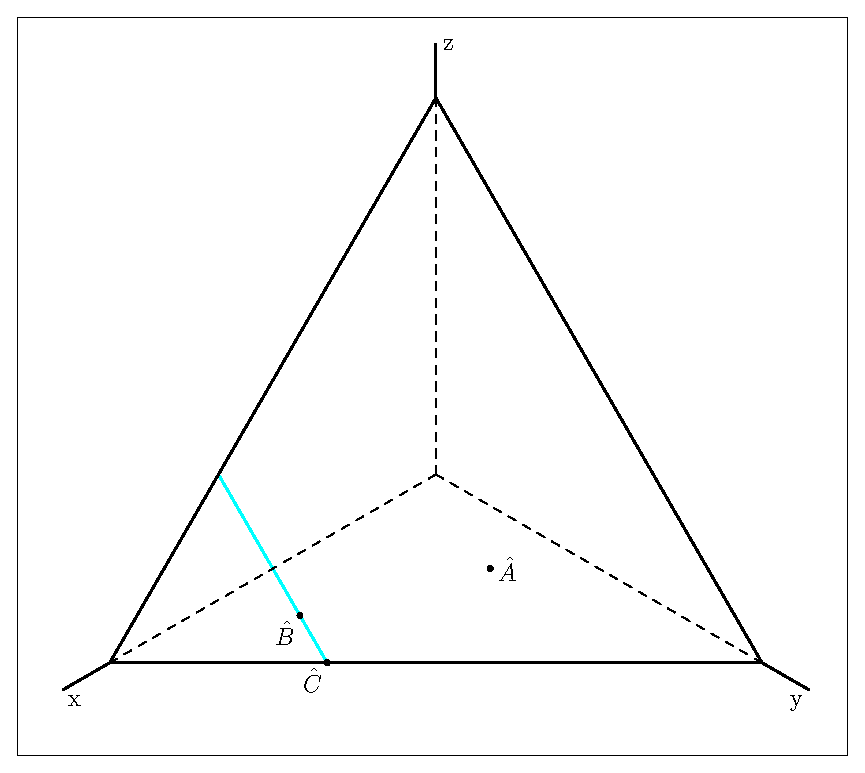
\includegraphics[width=\textwidth]{threepointshat.eps}
      \caption{\footnotesize The simplex $\mathbb{S}^{3}$ in
        three-dimensional space $\mathbb{R}^{3}$ with points
        $\hat{A},\hat{B},\hat{C}$ as in equation (\ref{eq:asy1}).
        Similar to figure (\ref{fig:threepoints}), $\hat{C}$ is closer
        to $\hat{A}$ than $\hat{B}$ is, geometrically speaking. Using
        the Kullback-Leibler divergence, however, $\hat{B}$ is closer
        to $\hat{A}$ than $\hat{C}$ is. The probability distribution
        corresponding to $\hat{B}$ is the Jeffrey posterior with
        respect to the probability distribution corresponding to
        $\hat{A}$. The probability distribution corresponding to
        $\hat{C}$ is the LP posterior and contains an extreme element.
        Jeffrey conditioning, by regularity, avoids extreme
        probabilities not required by the evidence. The coloured line
        going through $\hat{B}$ and $\hat{C}$ signifies the constraint
        that the evidence imposes on the posterior distribution,
        mandating that the $x$-coordinate must be $2/3$.}
      \label{fig:threepointshat}
    \end{minipage}
  \end{flushright}
\end{figure}

The Euclidean distance between $\hat{A}$ and $\hat{C}$ is smaller than
between $\hat{A}$ and $\hat{B}$.\tbd{See schmierbuch page 1470. It
  takes more information to go from a point with high entropy to a
  point with low entropy than vice versa. Why? Why does the geometry
  of reason fail to reflect this? In information theory, including is
  much easier than excluding. The geometry of reason portrays them to
  be equally easy or equally difficult.}

We are going to address two of Joyce's axioms that explicitly invoke
the geometry of reason and show how information theory agrees with one
of them while violating the other.

\begin{quotex}
  \textbf{Weak Convexity}: Let $m=(0.5b'+0.5b'')$ be the midpoint of the line
  segment between $b'$ and $b''$. If $I(b',\omega)=I(b'',\omega)$,
  then it will always be the case that $I(b',\omega)\geq{}I(m,\omega)$
  with identity only if $b'=b''$.
\end{quotex}

\begin{quotex}
  \textbf{Symmetry}: If $I(b',\omega)=I(b'',\omega)$, then for any
  $\lambda\in{}[0,1]$ one has\newline
  $I(\lambda{}b'+(1-\lambda)b'',\omega)=I((1-\lambda){}b'+\lambda{}b''),\omega)$.
\end{quotex}

The geometry of reason (certainly in its Euclidean form) mandates Weak
Convexity because the bisector of an isosceles triangle is always
shorter than the isosceles sides. It is not, in fact, only the
midpoint between $b'$ and $b''$ which will be less inaccurate with
respect to $\omega$ than either $b'$ or $b''$, but any point
$\lambda{}b'+(1-\lambda)b''$ with $0\leq\lambda\leq{}1$ (for the proof
see appendix \ref{app:wcs}).

Symmetry, on the other hand, fails for information theory. A simple
example, again for the three-dimensional case, is in figures
(\ref{fig:symmetrylp}), (\ref{fig:symmetryrj}), and
(\ref{fig:symmetrytgr})).

\begin{figure}[ht]
  \begin{flushright}
    \begin{minipage}[h]{.7\linewidth}
      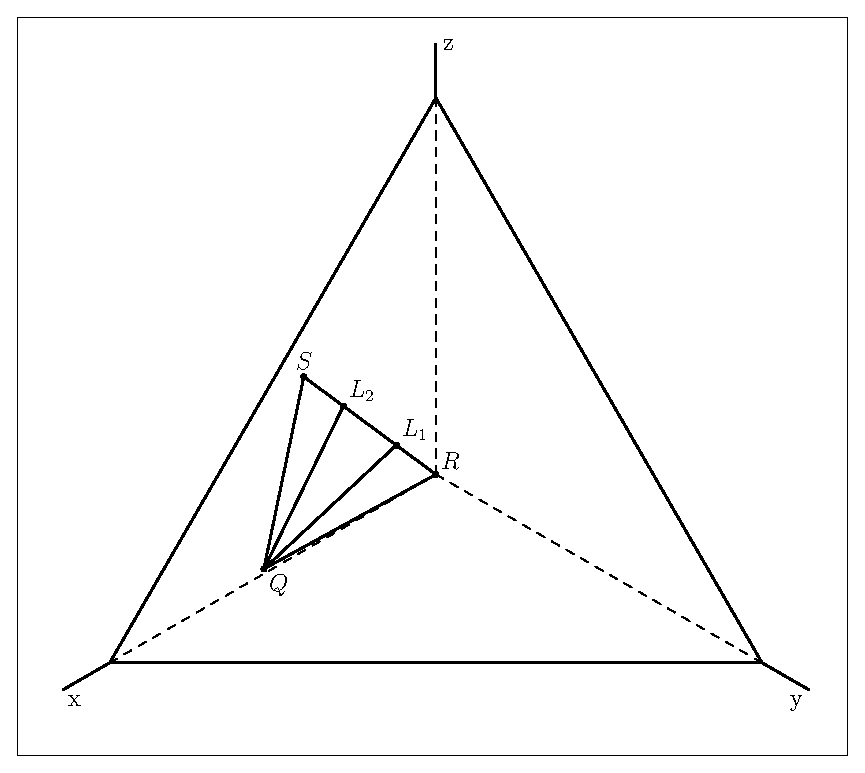
\includegraphics[width=\textwidth]{symmetrylp.eps}
      \caption{\footnotesize The simplex $\mathbb{S}^{3}$ in
        three-dimensional space $\mathbb{R}^{3}$ with points
        $Q,R,S,L_{1},L_{2}$, where $\|Q-R\|=\|Q-S\|$,
        $L_{1}=\lambda\Vec{OR}+(1-\lambda)\Vec{OS}$ and
        $L_{2}=(1-\lambda)\Vec{OR}+\lambda\Vec{OS}$. As you would
        expect with a Euclidean metric, $\|Q-L_{1}\|=\|Q-L_{2}\|$.}
      \label{fig:symmetrylp}
    \end{minipage}
  \end{flushright}
\end{figure}

\begin{figure}[ht]
  \begin{flushright}
    \begin{minipage}[h]{.7\linewidth}
      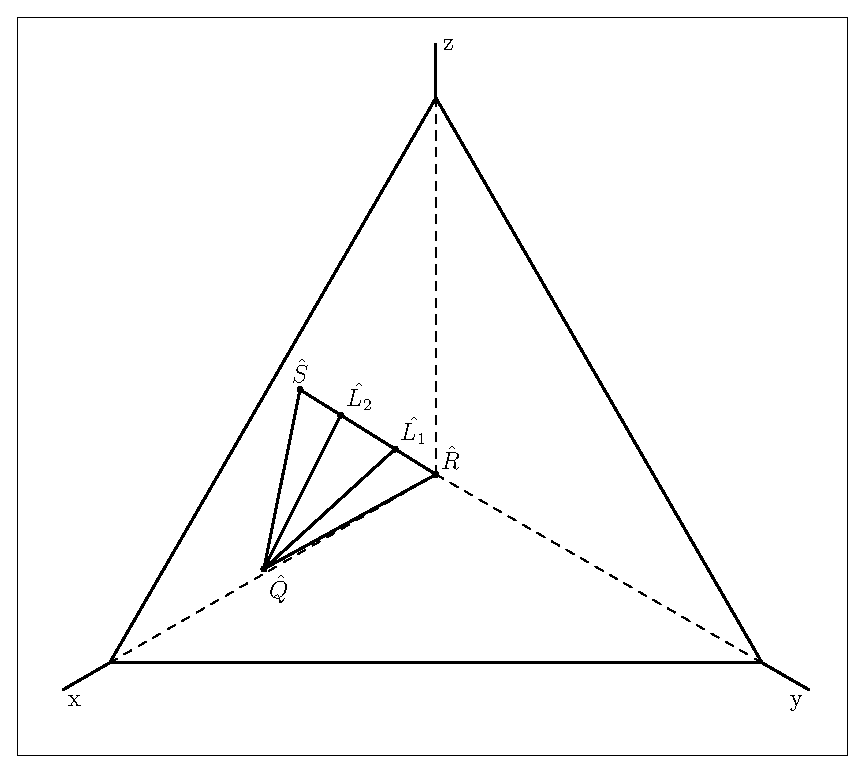
\includegraphics[width=\textwidth]{symmetryrj.eps}
      \caption{\footnotesize The simplex $\mathbb{S}^{3}$ in
        three-dimensional space $\mathbb{R}^{3}$ with points
        $\hat{Q},\hat{R},\hat{S},\hat{L_{1}},\hat{L_{2}}$, where
        $D_{\mbox{\tiny KL}}(\hat{Q},\hat{R})=D_{\mbox{\tiny
            KL}}(\hat{Q},\hat{S})$,
        $\hat{L_{1}}=\lambda\Vec{O\hat{R}}+(1-\lambda)\Vec{O\hat{S}}$
        and
        $\hat{L_{2}}=(1-\lambda)\Vec{O\hat{R}}+\lambda\Vec{O\hat{S}}$.
        However, in violation of Joycean symmetry, $D_{\mbox{\tiny
            KL}}(\hat{Q},\hat{L_{1}})\neq{}D_{\mbox{\tiny
            KL}}(\hat{Q},\hat{L_{2}})$.}
      \label{fig:symmetryrj}
    \end{minipage}
  \end{flushright}
\end{figure}

\begin{figure}[ht]
  \begin{flushright}
    \begin{minipage}[h]{.7\linewidth}
      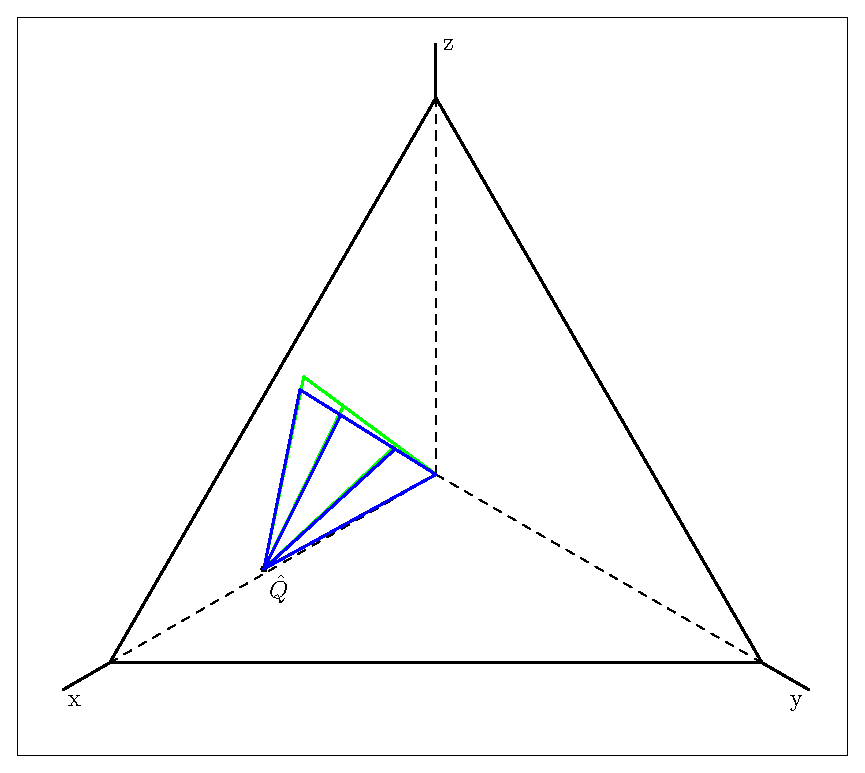
\includegraphics[width=\textwidth]{symmetrytgr.eps}
      \caption{\footnotesize Figure (\ref{fig:symmetrylp}) and figure
        (\ref{fig:symmetryrj}) superimposed in different colours to
        show that the \qnull{isosceles} triangles (\qnull{isosceles}
        with respect to Euclidean metric and Kullback-Leibler
        divergence respectively) are not congruent.}
      \label{fig:symmetrytgr}
    \end{minipage}
  \end{flushright}
\end{figure}

Another area where similarity measures are important is
multidimensional scaling (or MDS), for example in genetics (or for
dating apps). I have noticed, especially in genetics, that the MDS
literature has a similar bias towards symmetry than the
epistemological literature advocating the geometry of reason.
Biologists are often interested in the clustering of DNA samples in
order to establish relationships between genetics and biological
properties. The clustering needs to be based on some kind of
similarity measure, for example Euclidean metrics or the
Kullback-Leibler divergence (see \scite{7}{gentleman06}{}). The
Euclidean metric is often preferred because it is easily computed and
visualized, but some biologists have noted the significance of the
Kullback-Leibler divergence, especially when it is used in conjunction
with mutual information and dependence relationships between genetic
measurements. The asymmetry of the Kullback-Leibler divergence is then
often considered to be a nuisance. Biologists sometimes resort to a
symmetric form of the Kullback-Leibler divergence, such as the sum
$D_{\mbox{\tiny KL}}(X,Y)+D_{\mbox{\tiny KL}}(Y,X)$. I suspect that in
genetics, just as in concept similarity for Tversky and for our case
against the geometry of reason, it may be useful to discard the bias
against asymmetry and investigate how it may be useful to identify the
gene expressions that are central (from which it is harder to deviate
towards the periphery) and those that are peripheral.

\section{Conclusion}
\label{ascc}

Leitgeb and Pettigrew's reasoning to establish LP conditioning on the
basis of the geometry of reason is valid. Given the failure of LP
conditioning with respect to the five expectations, it cannot be
sound. The premise to reject is the geometry of reason. Fortunately,
information theory replaces it and yields results that fulfill the
five expectations.\tbd{(1) The heart piece of the paper is asymmetry.
  (2) This paper does not provide a complete axiomatization to justify
  probabilism, standard conditioning, and Jeffrey conditioning from an
  epistemic utility approach as Shore and Johnston have done from a
  pragmatic utility approach [?]. It is a potential future project to
  see how much of Joyce's results can be recovered after giving up on
  symmetry. (3) Incorporate Tversky and perhaps Cassirer. (4) Does the
  grade example imply asymmetry?}

\appendix

\section{Appendix: Weak Convexity and Symmetry in Information Geometry}
\label{app:wcs}

Using information theory instead of the geometry of reason, Joyce's
result still stands, vindicating probabilism on epistemic merits
rather than prudential ones: partial beliefs which violate probabilism
are dominated by partial beliefs which obey it, no matter what the
facts are.

Joyce's axioms, however, will need to be reformulated to accommodate
asymmetry. This appendix shows that the axiom Weak Convexity (see
section \ref{eugr}) still holds in information geometry. Consider
three points $Q,R,S\in\mathbb{S}^{n}$ (replace $\mathbb{S}^{n}$ by the
$n$-dimensional space of non-negative real numbers, if you do not want
to assume probabilism) for which

\begin{equation}
  \label{eq:app1}
  D_{\mbox{\tiny KL}}(Q,R)=D_{\mbox{\tiny KL}}(Q,S).
\end{equation}

I will show something slightly stronger than Weak Convexity: Joyce's
inequality is not only true for the midpoint between $R$ and $S$ but
for all points $\lambda{}R+(1-\lambda)S$, as long as
$0\leq\lambda\leq{}1$. The inequality aimed for is

\begin{equation}
  \label{eq:app2}
  D_{\mbox{\tiny KL}}(Q,\lambda{}R+(1-\lambda)S)\leq{}D_{\mbox{\tiny KL}}(Q,R)=D_{\mbox{\tiny KL}}(Q,S).
\end{equation}

To show that it holds I need the log-sum inequality, which is a result
of Jensen's inequality (for a proof of the log-sum inequality see
Theorem 2.7.1 in \scite{8}{coverthomas06}{31}). For non-negative
numbers $a_{1},\ldots,a_{n}$ and $b_{1},\ldots,b_{n}$,

\begin{equation}
  \label{eq:logsum}
  \sum_{i=1}^{n}a_{i}\ln\frac{a_{i}}{b_{i}}\geq\left(\sum_{i=1}^{n}a_{i}\right)\ln\frac{\sum_{i=1}^{n}a_{i}}{\sum_{i=1}^{n}b_{i}}.
\end{equation}

(\ref{eq:app2}) follows from (\ref{eq:logsum}) via

\begin{align}
  \label{eq:app3}
  &D_{\mbox{\tiny KL}}(Q,R)=\lambda{}D_{\mbox{\tiny KL}}(Q,R)+(1-\lambda)D_{\mbox{\tiny KL}}(Q,S)=\notag \\
  &\sum_{i=1}^{n}\left(\lambda{}q_{i}\ln\frac{\lambda{}q_{i}}{\lambda{}r_{i}}+(1-\lambda)q_{i}\ln\frac{(1-\lambda)q_{i}}{(1-\lambda)s_{i}}\right)\geq\notag \\
  &\sum_{i=1}^{n}q_{i}\ln\frac{q_{i}}{\lambda{}r_{i}+(1-\lambda)s_{i}}=D_{\mbox{\tiny KL}}(Q,\lambda{}R+(1-\lambda)S).
\end{align}

I owe some thanks to physicist friend Thomas Buchberger for help with
this proof. Interested readers can find a more general claim in
Csisz{\'a}r's Lemma 4.1 (see \scite{8}{csiszarshields04}{448}), which
accommodates convexity of the Kullback-Leibler divergence as a special
case.

\bibliographystyle{ChicagoReedweb} 
\bibliography{bib-2902}

\end{document}